







\section{Evaluation}
In this section we evaluate the implementation of our
approach across two case studies. 

These experiments aim at answering the following research questions:

1. RQ1: How do standard GCC optimization levels influence
on the resource consumption of running programs?
To answer this question, we apply standard optimization options to FFMPEG library. Then, we evaluate the memory footprint and execution time of running FFmpeg command lines and we
compare the results. The goal of this initial experiment is to
provide an understanding of the performance of
generated code by GCC.

2. RQ2: To what extent can the proposed diversity-based
exploration of optimization options impact the resource
consumption of running programs?
In a second experiment, we assess our novelty search
approach for automatic optimization sequences generation by
comparing the results founded by applying standard optimization sequences to new
results provided by our approach. In general, these experiments
show that our novelty-based approach produces optimization
sequences with higher performance and less resource consumption
than standard optimization levels in GCC. In this experiment, we focused as well on the tradeoff execution time/memory consumption.




\subsection{Case Study 1: FFMPEG}
In the first experiment, we set up our infrastructure for testing and monitoring the generated code. In this part, We compiled the FFMPEG library using standard GCC optimizations(O1, O2, O3, Ofast) and we studied the impact of these optimizations on memory consumption and execution time using our docker based infrastructure.

\subsubsection{FFMPEG: Multimedia Encoding Library}
FFmpeg is a complete, cross-platform solution to record, convert and stream audio and video. It is a very fast video and audio converter. It processes a number of input files specified by the $-i$ option, and generate different output files according to the input plugin. FFmpeg allows different types of video conversion and that depends on the input and output format (video, audio, subtitle, attachment, data).
Some command options have to be specified for each type of video or audio processing. In fact,
FFmpeg defines a set of option flags through command line to configure and generate the output
file (e.g. number of threads, size, bitrate, the video or audio codec). Video or audio processing with FFmpeg consumes lot of resources in term of memory usage. So, testing GCC on top of this library is very interesting. 
\subsubsection{Docker-based Infrastructure for monitoring FFmpeg containers}
\begin{figure}[h]
	\centering
	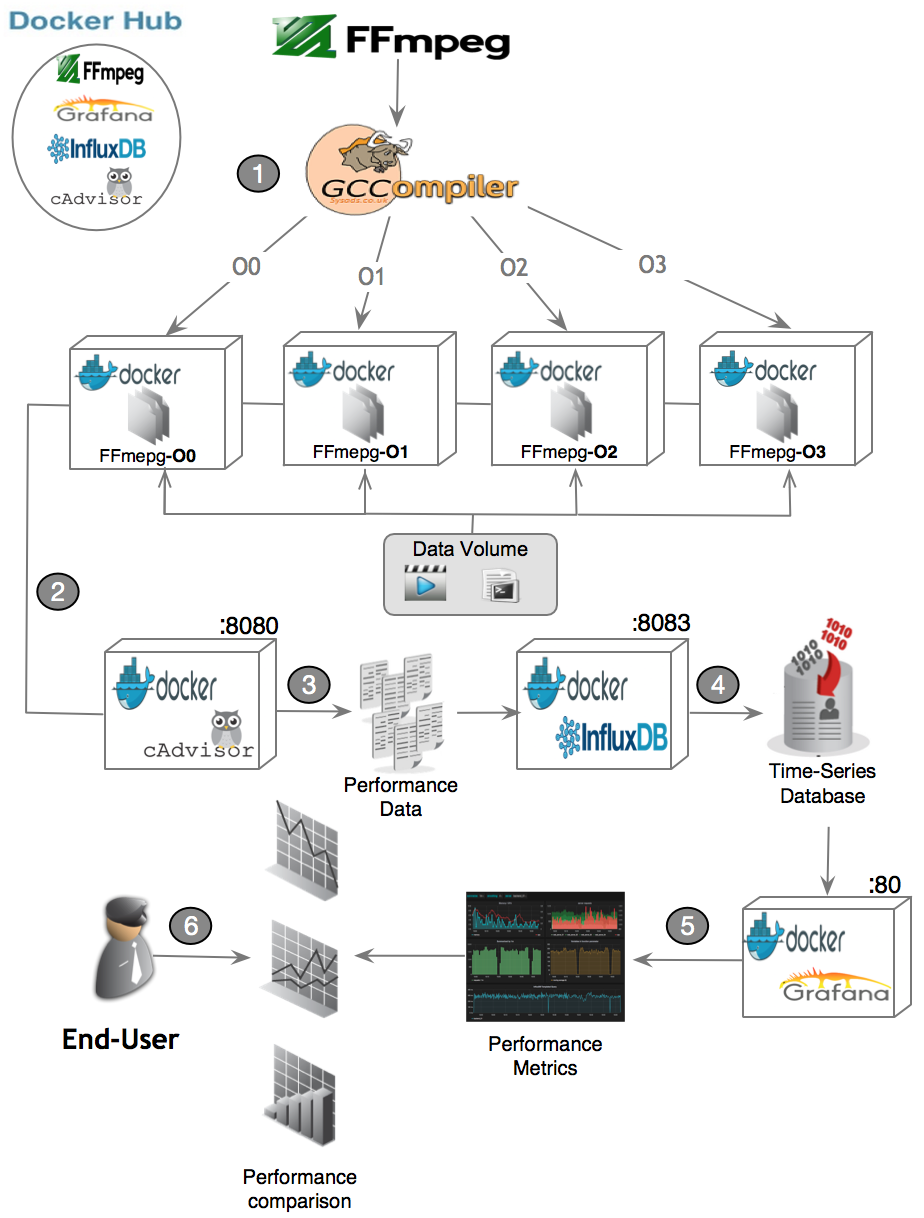
\includegraphics[scale=0.40]{infra_ffmpeg.png}
	\caption{Overview of the different components involved in testing and monitoring of FFMPEG containers}
\end{figure}
\begin{figure*}
	
	\center
	
	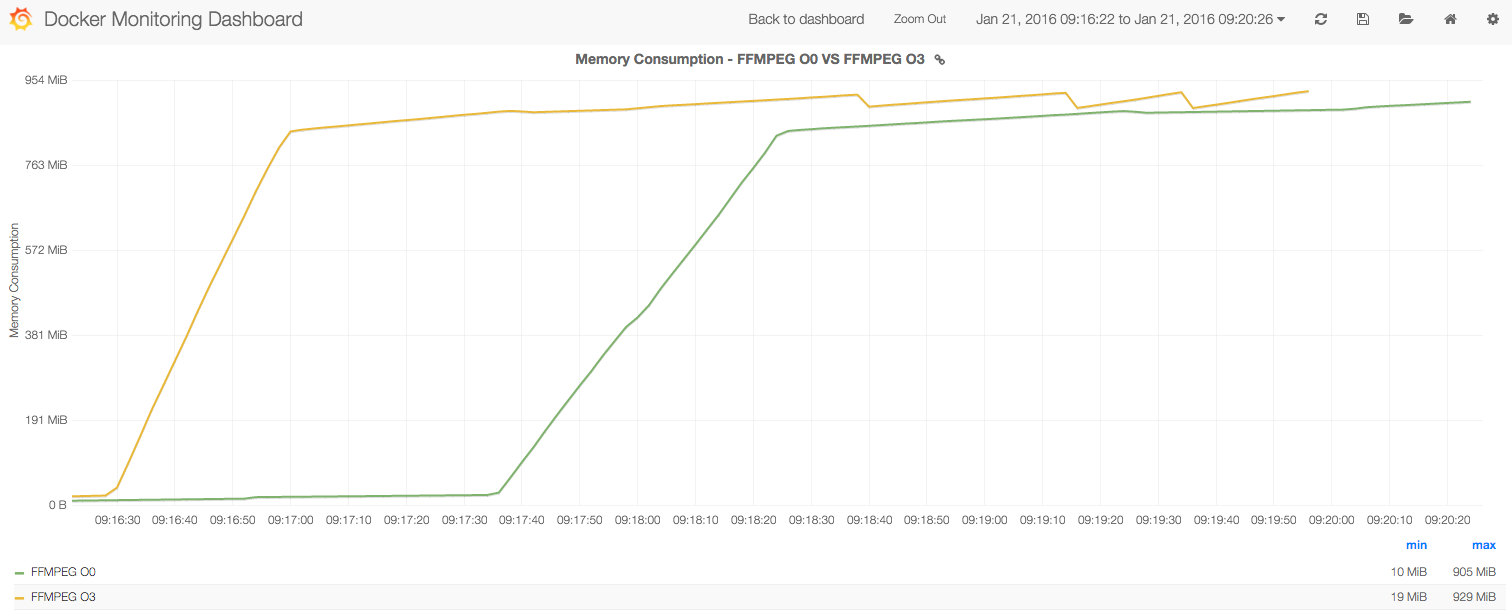
\includegraphics[width=15cm,height=6cm]{infra_stats.png}
	\caption{Runtime memory consumption profiles of workload running in FFMPEG containers compiled with O0 (no optimization) and O3 options}
	
	\label{AAA}
	
\end{figure*}
The goal of this experiment is to compile FFmpeg with standard GCC optimization options and run FFmpeg command examples on different versions in order to compare the memory usage profiles and execution time of different variants using our testing architecture. An overview of the different components involved in testing and monitoring of FFmpeg containers is shwon in Figure 2. 
First, we compile FFmpeg library with different optimization options  (O0, O1, O2, O3 and Ofast) in order to produce 5 variants of FFmpeg. This is done within a Docker container with a Linux image. We configure
each container to install FFmpeg with a specific configuration and we uploaded all the FFmpeg images in Docker Hub.
Docker Hub is a cloud-based registry service for building and shipping application or
service containers. We are using it for building, saving and managing all our docker
images.
 Then, we execute the same ffmpeg testing examples within each ffmpeg instance container. We choose 15 ffmpeg example commands that cover multiple domains[ref blog] like video conversion, sound extraction, encoding file for iPod or PSP, etc. This list of examples is saved in a script file to execute within containers. The media files needed for encoding are saved in a shared repository. In Docker environment, we call this repository the “Data Volume”. A data volume is a specially-designated directory within containers that share data with the host machine. Data is persistent and independent of container’s life cycle. So, when we run FFmpeg containers we provide a shared volume with the host
machine (where the media files are located). As well, the list of ffmpeg commands to execute is mounted in this volume so that we can execute the same workload for each container.

Before running the FFmepg workload on different containers, we run monitoring components (cAdvisor, InfluxDB and Grafana) to start gathering usage statistics.

Using Grafana, we are able to query database and define performance metrics. We use for this experiment to gather statistics about memory consumption and execution time of different containers. 

\subsubsection{Experimental results}

The first part of this experiment is to compare the no-optimization container with the high-optimization one in order to study the impact of optimizations on resource consumption. Figure 3 shows runtime statistics for two running ffmpeg containers O0 and O3 with the same input workload. This chart present the memory usage profile of two components (FFMPEG O0 and O3) started in the same time and running in parallel. Visually, we can see that the execution of O3 (yellow) is faster than O0 (green) by around 20s. However, we can see that memory usage remains higher than O0 from the beginning to the end of running the ffmpeg examples. 

To better understand resource usage of optimized containers, we run the same experiment for all ffmpeg containers and we collected the same metrics. Figure 4 presents a comparison of average memory usage and execution time of FFmpeg containers compiled with all standard GCC optimization options. We remark that the memory usage is increasing as soon as we apply more aggressive optimization.

This results explain that optimizing for execution time (for the case of ffmpeg) is not always efficient regarding memory usage and unfortunately, optimizations may influence negatively on system resources. 
\begin{figure}[h]
	\centering
	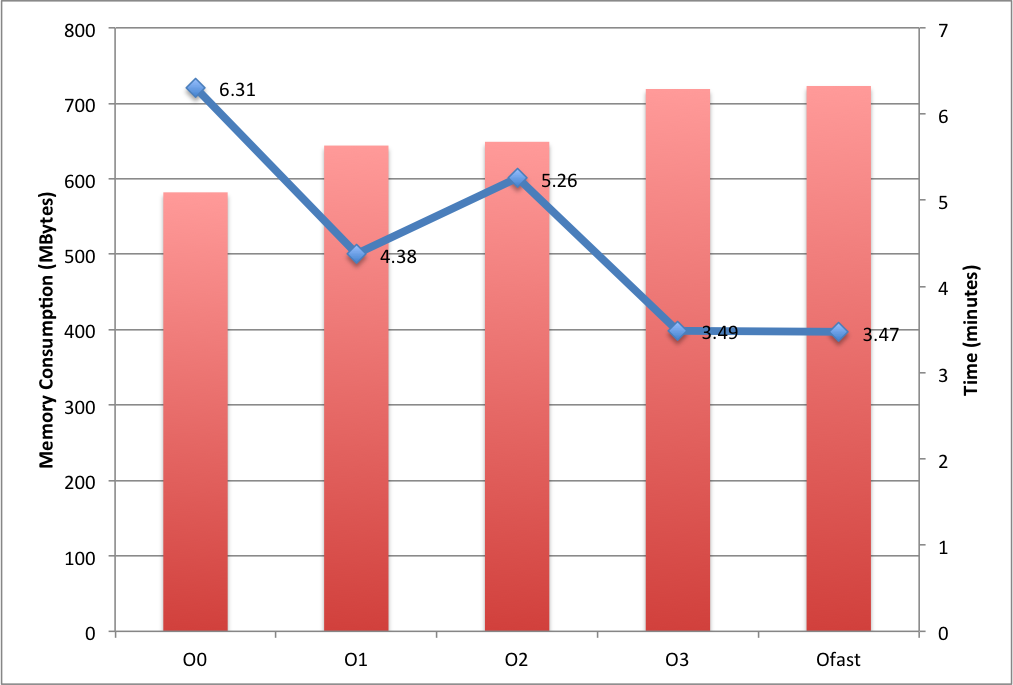
\includegraphics[scale=0.4]{infra_ffmpeg_plot1.png}
	\caption{Comparison of average memory consumption and execution time of running workload in FFMPEG containers compiled with standard GCC optimization options}
\end{figure}






\subsection{Case Study 2: Novelty-based exploration of optimization sequences}
For the second experiment, we present a set of experiments to evaluate the performance optimized programs across target benchmarks. The goal of this section
is to show that our approach for exploring the search space of optimizations is able to generate efficient sequences of optimization options in term of performance and
resource consumption. We define an efficient sequence as a
set of optimization options that induce to low consumption of
memory and CPU resources.
\subsubsection{Benchmark programs}
To explore the impact of compiler optimizations a set of test input programs are needed. We run experiments on commonly used benchmarks named Collective Benchmark (cBench). It is a collection of open-source sequential programs in C targeting specific areas of the embedded market. It comes with multiple datasets assembled by the community to enable realistic benchmarking and research on program and architecture optimization. cBench contains more than 20 C programs. The following table describes programs that we have selected from this benchmark.
\begin{table}[h]
	\begin{center}
		\begin{tabular}{|c|c|p{4cm}|}
			\hline
			\textbf{Program} & \textbf{Source lines} & \textbf{Description}\\
			\hline
			automative-susan-s & 1376 & Image recognition package\\
			\hline
			bzip2e & 5125 & Compress any any file
			source code \\
			\hline
			bzip2d & 5125 & Decompress zipped files \\
			\hline
			office-rsynth & 4111 & Text to speech program produced by integrating various pieces of code\\
			\hline
			 &  & \\
			
			\hline
			 & & \\
			\hline
			
		\end{tabular}
		
	\end{center}
	\caption {Description of selected benchmark programs}
\end{table}
\subsubsection{Novelty Parameters}
Our experiments use the classical Novelty Search algorithm, where we evolve a set of optimization sequences through generations.
Novelty search is implemented as described in Section X.

The first step in the process of selection is to evaluate each individual and compute its novelty score. Novelty is calculated for each organism by taking the mean of its 15 lowest dissimilar optimization sequences, by considering all sequences in the current population and in the archive. 

Then, to create next populations, an elite of the 10 most novel organisms is copied unchanged, after which the rest of the new population is created by tournament selection according to novelty. Standard genetic programming crossover and mutation operators are applied to these novel sequences in order to produce offspring individuals and fulfill the next population.

In the meanwhile, individuals that get a score higher than the threshold T they are automatically added to the archive as well. 

In fact, this threshold is dynamic. Every 1500 evaluations, it is checked how many individuals have been copied into the archive. If this number is below 3, the threshold is increased by multiplying it by 0.95, whereas if solutions added to archive are above 3, the threshold is decreased by multiplying it by 1.05. 

Moreover, as the size of the archive grows, the nearest-neighbor calculations that determine the novelty scores for individuals become more computationally demanding. So to avoid having low accuracy of novelty, we choose to bound the size of the archive. Hence, it follows a queue data structure (first-in first-out) which means that when a new solution gets added (enqueued), the oldest solution in the novelty archive will be discarded or dequeued. Thus, we ensure individuals diversity by removing old sequences that may no longer be reachable from the current population.

The parameters of the algorithm were tuned individually in preliminary experiments. For each parameter, a set of values was tested. The parameter values chosen are the mostly used in the literature. The value that yielded the highest performance scores was chosen. The resulting parameter values are listed in Table 2.
\begin{table}
	\begin{center}
		\caption{Parameters of the evolutionary algorithm}
		\begin{tabular}{ l l || l l }
			Parameter & Value & Parameter & Value \\	\hline
			Novelty nearest-k  & 15 &  Tournament size & 2\\ 
			Add archive prob. & 30 &  Mutation prob. & 0.1\\  
			Max archive size & 500 &  Crossover & 0.5  \\  
			Population size & 100 &  No generations &  1000 \\  
			Individual length & 76 & Elitism & 10  \\ 
			Scaling archive prob. & 0.05 & New in archive z & 3  \\ 
		\end{tabular}
	\end{center}
\end{table}

\begin{figure}[h]
	\centering
	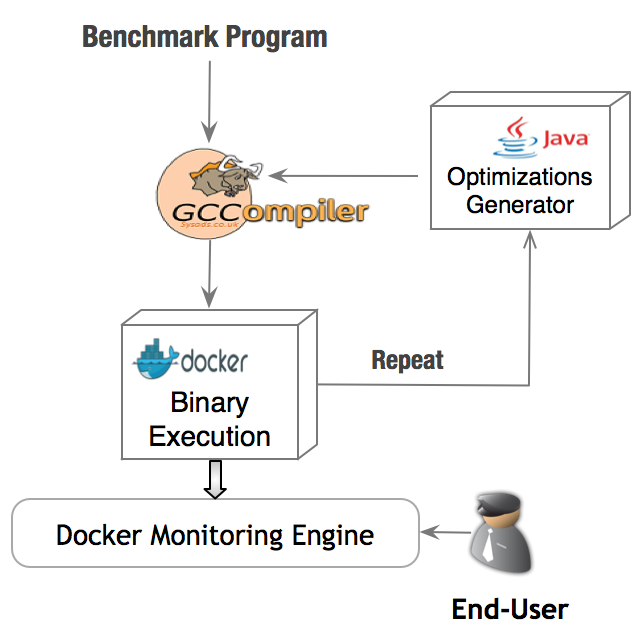
\includegraphics[scale=0.50]{infra_novelty.png}
	\caption{Overall process of optimization space exploration and monitoring}
\end{figure}

\begin{figure}[h]
	\centering
	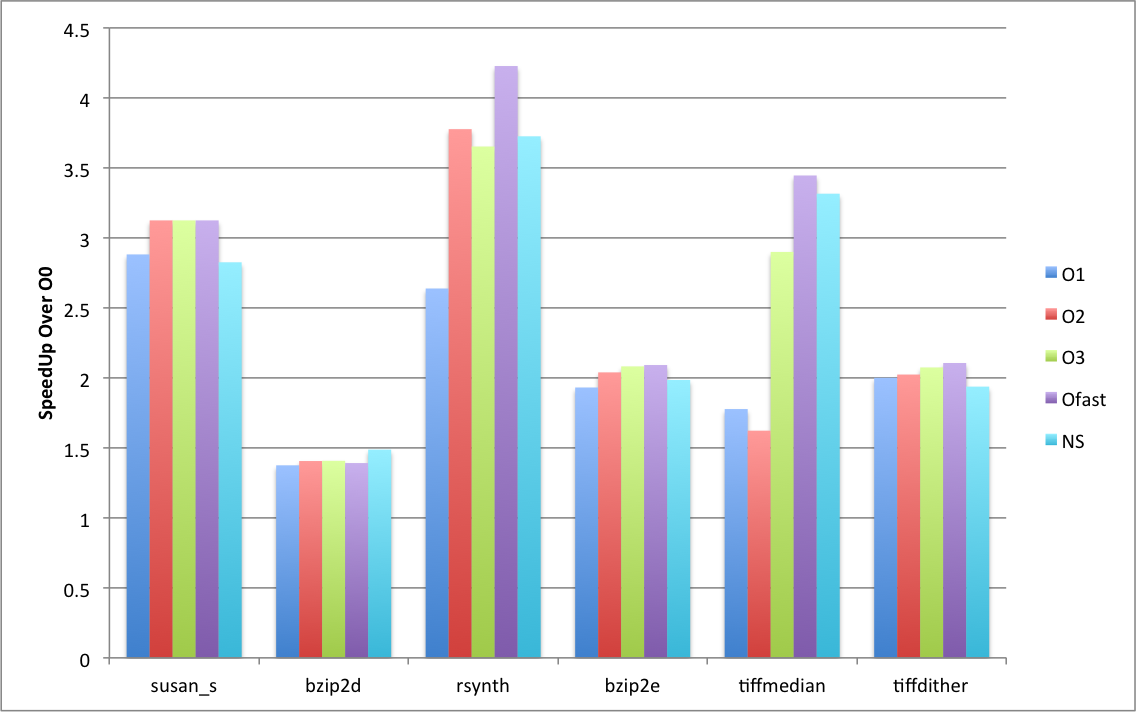
\includegraphics[scale=0.50]{infra_novelty_stat2.png}
	\caption{Evaluating the speedup after applying standard optimization options comparing to new generated optimizations using Novelty Search}
\end{figure}
\begin{figure}[h]
	\centering
	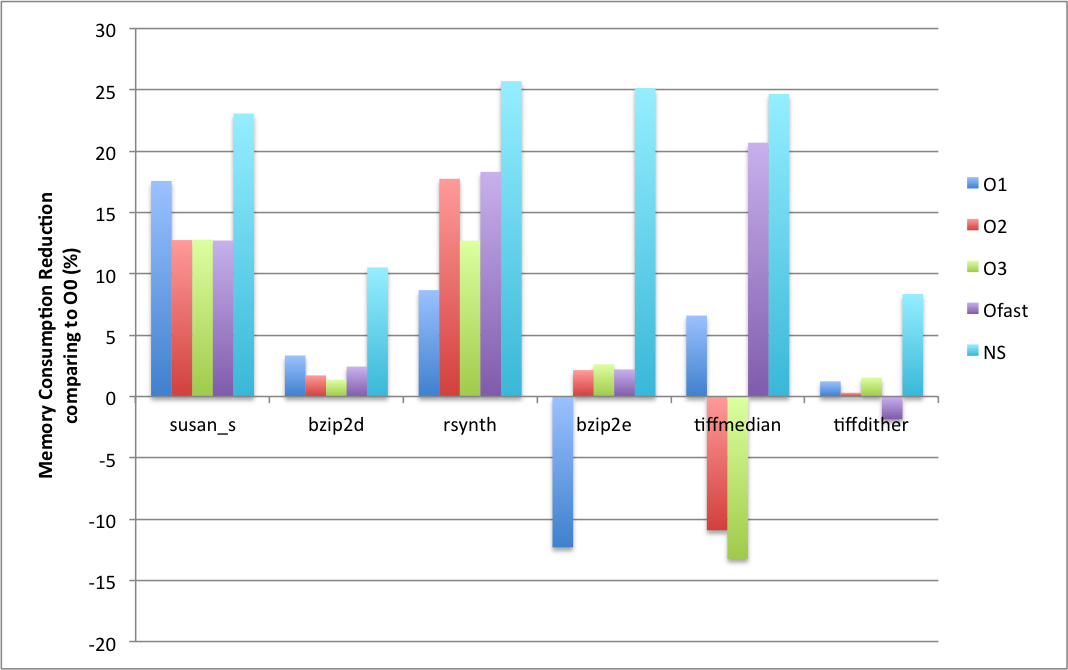
\includegraphics[scale=0.50]{infra_novelty_stat3.png}
	\caption{Evaluating the amount of saved memory after applying standard optimization options comparing to new generated optimizations using Novelty Search}
\end{figure}

\section{Related Work}
\section{Conclusion and Future work}